\documentclass[12pt]{article}


% for less space at the sides
\usepackage{a4wide}
% to display headings in german
\usepackage{ngerman}
% to corecctly display umlauts
\usepackage[utf8]{inputenc}
% for designing my own header
\usepackage{fancyhdr}
% to use colors by name
\usepackage[usenames,dvipsnames]{color}
\usepackage{subcaption}
\usepackage{xfrac}
\usepackage{url}

\usepackage{amsmath}
\usepackage{amssymb}
\usepackage{enumerate}
\usepackage{enumitem}
\usepackage{cancel}
\usepackage{graphicx}
\usepackage{float}
\usepackage{tabularx}
\usepackage{tikz}
\usepackage{svg}
\usepackage{listings}



\newcommand{\N}{\mathbb{N}}
\newcommand{\Z}{\mathbb{Z}}
\newcommand{\Q}{\mathbb{Q}}
\newcommand{\R}{\mathbb{R}}
\newcommand{\C}{\mathbb{C}}



\newcommand{\highlight}[1]{\textcolor{Blue}{\textbf{\textit{#1}}}}
\newcommand{\emphasize}[1]{\textcolor{Gray}{\textit{#1}}}
\newcommand{\runtime}[1]{\textcolor{Red}{\textbf{#1}}}
\newcommand{\headline}[1]{\vspace{15pt}\textbf{#1}\vspace{10pt}}
\newcommand{\code}[1]{\textcolor{Green}{\texttt{#1}}}
\usepackage[boxed]{algorithm2e}
\lstset{
basicstyle=\footnotesize,
frame=single
}


\setlength{\parindent}{0pt}

% definition of the header
\pagestyle{fancy}
\fancyhead{}
\fancyfoot{}
\fancyhead[LO, LE]{Deep Learning}
\fancyhead[RE, RO]{\today}
\fancyhead[C]{\slshape Seite \thepage}

\title{Deep Learning}
\begin{document}
	\begin{titlepage}
%-------------------------------------------------------------
		\begin{center}
			{\Large\bf Netzoptimierung und Lernalgorithmen für Neuronale Netze}\\[2cm]

			{\bf Master}\\
			zur Erlangung des Grades {\em Master of Science}\\[1.5cm]

			an der\\
			Hochschule Niederrhein\\
			Fachbereich Elektrotechnik und Informatik\\
			Studiengang {\em Informatik}\\[3cm]

			vorgelegt von\\
			Michael Kämmerer\\
			805467 \\[3cm]
			Datum: \today\\[3cm]

			Prüfer: Prof.~Dr.~Peer Ueberholz\\
			Zweitprüfer: Prof.~Dr.~Christopher Dalitz
		\end{center}
	\end{titlepage}
	
	\begin{titlepage}
%-------------------------------------------------------------

\section*{Eidesstattliche Erklärung}
\subsubsection*{Schriftliche Abschlussarbeit}

des Studenten: Michael Kämmerer\\
Matrikelnummer: 805467\\



Thema: {\em Netzoptimierung und Lernalgorithmen für Neuronale Netze} \newline

\textbf{Ich versichere durch meine Unterschrift, dass die vorliegende Abschlussarbeit 
 ausschließlich von mir verfasst bzw. angefertigt wurde. Es wurden keine anderen als die 
  angegebenen Quellen und Hilfsmittel benutzt.}

Betreuender Dozent:  Prof. Dr. Peer Ueberholz

Krefeld, den {\em \today}

\begin{tabular}{l}
\\
\\
\hline
(Michael Kämmerer)\\
\end{tabular}

\newpage
\end{titlepage}

	\newpage

	\tableofcontents
	
	\newpage
	\section{Einleitung}
	Seit jeher wird versprochen, dass der Computer das Leben des Menschen einfacher machen soll und diesem alle Arbeit abnehmen können wird. In vielen Bereichen funktioniert dies schon sehr gut, jedoch scheitern Computer immer noch an sehr einfachen Aufgaben. Menschen können problemlos unterscheiden, ob ein Hund oder eine Katze auf sie zugelaufen kommt oder ein Tier als Katze identifizieren ohne genau die Rasse zu kennen. Menschen können trainierte Fähigkeiten mühelos auf neue Aufgaben übertragen und anwenden.
	Ein Versuch diese Fähigkeiten nachzubilden stellen künstliche neuronale Netze dar. Diese sind ein Teilgebiet der künstlichen Intelligenz und versuchen die Arbeitsweisen des menschlichen Gehirns nachzubilden. Diese sollen durch Lernen Lösungen zu bestimmten Problemen finden und auf andere Probleme anwenden können. Ein großes Feld für diese Probleme ist die Mustererkennung und Einordnung von Bildern, um die es auch in dieser Arbeit geht. 
	
	Die Forschungen zu neuronalen Netze wurden 1969 durch eine Veröffentlichung von Marvin Minsky und Seymour Papert fast völlig eingestellt, da diese gezeigt haben, dass diese Netze nicht einmal einfache Aufgaben lösen können. Wie man später herausfand, lag diese Fehlaussage darin begründet, dass die beiden nur ein einlagiges Netz untersuchten. Ein erster großer Durchbruch bei neuronalen Netzwerken stellt die Entwicklung des Backpropagation-Algorithmus durch Paul Werbos im Jahre 1974 dar. Dieser ermöglicht das einfache Trainieren von mehrlagigen neuronalen Netzen. Dieser Algorithmus liefert gute Ergebnisse wenn die neuronalen Netze wenige Schichten haben, allerdings nimmt die Laufzeit für jede neue Schicht sehr stark zu. Da die Anzahl der Neuronen auf jeder Ebene bestimmt, wie viele Parameter erkannt werden können, führte dies zu sehr breiten und Flachen neuronalen Netzen die erforscht wurden.
	
	Ein weitere Durchbruch gelang Geoffrey Hinton und Yee-Whye Teh im Jahre 2006, als diesen die kontrastive Divergenz zum Trainieren von neuronalen Netzen  vorstellten. Dieser Algorithmus erlaubte es sehr effizient neuronale Netze mit vielen Schichten zu trainieren, die sogenannten Deep-Belief Netze. Nun war es einfach möglich, mit jeder neuen Schicht in einem neuronalen Netzwerk weitere Eigenschaften des zu erlernenden Problems zu erkennen und die Lösung zu verbessern. 
	
	Diese Arbeit beschäftigt sich mit Deep-Belief Netzen und verschiedenen Möglichkeiten mit ihnen Bilder zu klassifizieren. Kapitel \ref{Grundlagen} erläutert dem Leser die benötigten Grundlagen für die Arbeit. Dazu gehören die Funktionsweise von neuronalen Netzen, der Backpropagation-Algorithmus, Markov-Ketten, Hopfield Netze, Boltzmann Maschinen, eingeschränkte Boltzmann Maschinen und die kontrastive Divergenz. Im Anschluss daran werden in Kapitel 3 Deep-Belief Netze vorgestellt und wie diese trainiert werden mit einer anschließenden Erläuterung wie man mit ihnen Bilder klassifiziert. In Kapitel 4 wird das benutzte Framework vorgestellt und welche Erweiterungen an diesem vorgenommen wurden. Kapitel 5 stellt die durchgeführten Versuche und die Ergebnisse vor. In Kapitel 6 wird darauf eingegangen, welche Probleme es bei Deep-Belief Netzen noch gibt und überlegt wie man diese in Zukunft noch verbessern könnte. 

	\section{Grundlagen}
	\label{Grundlagen}
	Als Grundlage für Deep-Belief Netze dienen eingeschränkte Boltzmann Maschinen. Diese sind eng mit Hopfield Netzen verwandt und der Weg von Hopfield Netzen zu eingeschränkten Boltzmann Maschinen wird in diesem Kapitel vorgestellt. Hopfield Netze und allgemeine Boltzmann Maschinen werden hierbei jedoch nur kurz erläutert und am Ende des Kapitels werden eingeschränkte Boltzmann Maschinen ausführlich erklärt. Die Kapitel \ref{NN} und \ref{BP} wurden aus meiner Bachelorarbeit \cite{bachelor} übernommen.
	\subsection{Künstliche neuronale Netze}
	\label{NN}
		Als Grundlage für künstliche neuronale Netze wird das Modell von Nervenzellen verwendet. Ein Neuron besteht aus einem Zellkörper, welcher mit Dendriten und einem Axon verbunden ist (siehe Abbildung \ref{Neuron}). Dendriten haben die Aufgabe, die Signale anderer Nervenzellen zu empfangen und zusammenzuführen, um diese als Eingabe in die Nervenzelle weiter zu geben. Der Zellkörper interpretiert die Eingabe und schickt die daraus resultierende Ausgabe über sein Axon. Das Axon ist mit Synapsen an die Dendriten anderer Nervenzellen gekoppelt (Nicht abgebildet)\footnote{http://de.wikipedia.org/w/index.php?title=Nervenzelle\&stableid=119646035}.
\begin{figure}[H]
	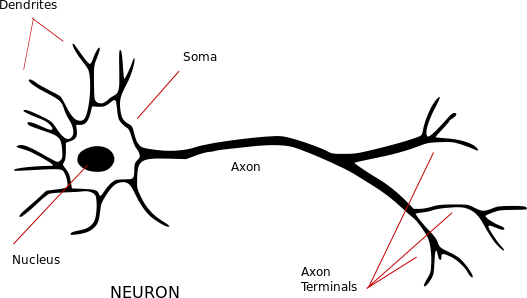
\includegraphics[scale=0.8]{Neuron_-_annotated.png}
	\caption{Neuron (Quelle: http://commons.wikimedia.org/wiki/File:Neuron\_-\_annotated.svg) }
	\label{Neuron}
\end{figure}		
		
	Naturwissenschaftlich werden Modelle entwickelt um Lernvorgänge im Gehirn zu beschreiben. Diese Modelle sind auch in der Informatik interessant. Alle Modelle haben dabei gemeinsam, dass sich über die Zeit hinweg eine hohe Fehlertoleranz und Robustheit gegen Störungen einstellt. Aus diesen Gründen werden künstliche neuronale Netze in der Informatik eingesetzt.
	 Desweiteren ermöglichen künstliche neuronale Netze Dinge assoziativ zu speichern. Dies ist natürlich mit Nachteilen verbunden, so braucht das neuronale Netz einen hohen Zeitaufwand um etwas zu lernen. Zusätzlich gibt es keine Garantie dafür, dass überhaupt richtig gelernt wurde. Als Einsatzgebiet für neuronale Netze eignen sich Entscheidungsprobleme, Roboter, Mustererkennung, Spracherkennung und überall, wo man sich eine künstliche Intelligenz vorstellen kann \cite{PDP}.
	
	Künstliche neuronale Netze bestehen aus Neuronen, die über Synapsen miteinander verbunden sind. Ein Neuron kann einen oder mehr Eingänge besitzen. Die Signale auf den Eingängen werden in der Regel aufsummiert und ergeben einen Gesamtinput $net_i$. Dadurch erhält das Neuron einen Aktivitätswert $a_i$ aus dem ein Ausgangswert $o_i$ folgt. Dieser Ausgangswert kann nun entweder gemessen werden oder das Neuron ist über eine oder mehrere Synapsen, die eine gewichtete Verbindung $w_{i,j}$ darstellt, an ein weiteres Neuron gekoppelt (Abbildung \ref{2n}) \cite{PDP}.
	
\begin{figure}[H]
	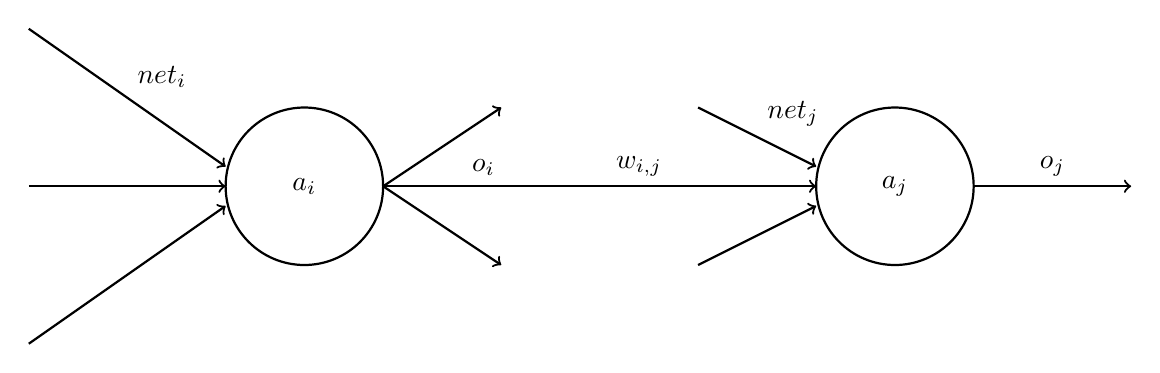
\begin{tikzpicture}	
	\draw[->,thick](0,0)--(2.5,0);
	\draw[->,thick](0,2)--(2.5,0.25)node[above right, midway]{$net_i$};
	\draw[->, thick](0,-2)--(2.5,-0.25);
	\draw[thick](3.5,0)circle(1) node{$a_i$};
	\draw[thick](4.5,0)--(5.5,0)node[above right]{$o_i$};
	\draw[->,thick](4.5,0)--(6,1);
	\draw[->,thick](4.5,0)--(6,-1);
	\draw[->,thick](5.5,0)--(10,0)node[midway, above]{$w_{i,j}$};
	\draw[->,thick](8.5,1)--(10,0.25)node[above right, midway]{$net_j$};
	\draw[->,thick](8.5,-1)--(10,-0.25);
	\draw[thick](11,0)circle(1) node{$a_j$};
	\draw[thick,->](12,0)--(14,0) node[above,midway]{$o_j$};
	\end{tikzpicture}
	\caption{Zwei miteinander verbundene Neuronen in einem Neuronalen Netz}
	\label{2n}
\end{figure}

	Zu diesem einfachen Modell des Aufbaus gibt es ein mathematisches Modell für die Funktionsweise von neuronalen Netzen. Dieses Modell kennzeichnet sich durch folgende Eigenschaften:
	
	\begin{enumerate}
		\item Jedes Neuron hat einen Aktivierungszustand $a_i(t)$ zum Zeitpunkt $t$.
		\item Jedes Neuron hat eine Aktivierungsfunktion $f_{act}$. Diese gibt an, wie sich die Aktivierung in Abhängigkeit der alten Aktivierung $a_i(t)$, des Inputs $net_i$ und eines Schwellwerts $\theta$ mit der Zeit ändert.
\begin{equation}a_i(t+1)=f_{act}(a_i(t),net_i(t),\theta)\end{equation}
		\item Jedes Neuron hat eine Ausgabefunktion $f_{out}$, die aus der Aktivierung den Output $o$ berechnet.
\begin{equation}o_i=f_{out}(a_i)\end{equation}
		\item Es existiert ein Verbindungsnetzwerk, dass aus den Synapsen $w_{i,j}$ besteht.
		\item Jedes Neuron hat eine Propagierungsfunktion, die aus den Ausgaben der anderen Neuronen die Netzeingabe berechnet. Diese lautet zumeist
\begin{equation}net_j(t)=\sum o_i(t)w_{i,j}.\end{equation}
		\item Eine Lernregel. Diese kann zum Beispiel daraus bestehen, die Ausgabe des Netzes mit einer gewünschten Ausgabe zu vergleichen um dann die Gewichte des Netzes anzupassen.
	\end{enumerate}
Die Zustände des neuronalen Netzes werden solange geändert, bis ein stabiler Endzustand eintritt. Dieser muss jedoch nicht das gewünschte Ergebnis liefern, in diesem Fall hätte das neuronale Netz falsch gelernt.\cite{PDP}
Im Folgenden wird nur der Fall $a_i=f_{act}(net_i)$ und $o_i=a_i$ betrachtet. Zusammengefasst erhält man so:
	\begin{equation}
	o_i=f_{act}(net_i)	
	\end{equation}

\subsection{Backpropagation-Algorithmus}
\label{BP}
	
	Damit das neuronale Netz seine Aufgabe erfüllen kann, muss es zunächst lernen. Dabei gibt es keine Einschränkung, wie gelernt werden kann. Es können neue Verbindungen oder Neuronen erstellt oder gelöscht werden, die Parameter der Neuronen angepasst werden oder die Stärke der Verbindungen geändert werden. Meistens wird die Modifikation der Verbindungsstärke gewählt, da dieses Lernverfahren am einfachsten ist. Alle in dieser Arbeit vorgestellten neuronalen Netze verwenden die Modifikation der Gewichtsstärken zum Lernen. Desweiteren wird zwischen drei Lernverfahren unterschieden:
	\begin{enumerate}
		\item {\bf Überwachtes Lernen:} Es existiert zu jedem Input ein gewünschter Output. Dieser wird mit dem tatsächlichen Output verglichen und das Netz angepasst.
		\item {\bf Bestärkendes Lernen:} Bei einem Input wird der Output auf richtig oder falsch überprüft. Mithilfe dieser Information wird das Netz angepasst.
		\item {\bf Unüberwachtes Lernen:} Das Netz organisiert sich selbstständig.
	\end{enumerate}
	
	Am häufigsten wird das überwachte Lernen verwendet. Es existieren verschiedene Methoden um dieses zu realisieren. Da für diese Arbeit jedoch nur das Back-Propagation-Verfahren eine Rolle spielt, wird nur dieses Verfahren genauer erläutert \cite{PDP}.
	
	Das Back-Propagation-Verfahren (BP) minimiert mithilfe eines Gradienten eine Fehlerfunktion. Diese wird meistens als Summe über die quadratische Abweichung des Outputs $o_{p,j}$ und des gewünschten Outputs $\hat{o}_{p,j}$ für ein Pattern(Event) $p$ definiert.
\begin{equation} 
	E=\sum_p^n E_p 
\end{equation}
\begin{equation}
	\label{fehler}
	E_p=\frac{1}{2}\sum_j^m(o_{p,j}-\hat{o}_{p,j})^2
\end{equation}
	
Hierbei ist $n$ die Anzahl der Pattern und $m$ die Anzahl der Outputs.
Mit Gleichung \ref{anpassung} versucht man die Gewichte entlang des Gradienten der Fehlerfunktion zu ändern, bis diese minimiert ist. Im optimalen Fall findet man damit das globale Minimum der Fehlerfunktion, meistens findet man jedoch nur ein lokales Minimum. 
\begin{equation}
\label{anpassung}
\Delta w_{ij}=-\eta\sum_p^m \frac{\partial E_p}{\partial w_{ij}}
\end{equation}
$\eta$ ist die Lernrate. Diese ist wichtig, um steuern zu können wie stark die Gewichte angepasst werden. Mit Hilfe der Kettenregel kann man die Formel umschreiben und auf zwei Faktoren reduzieren:
\begin{equation}
\Delta w_{ij}=\eta\sum_p^m -\frac{\partial E_p}{\partial net_{pj}}\frac{\partial net_{pj}}{\partial w_{i_j}}
\end{equation}

Der erste Faktor wird als Fehlersignal $\delta_{pj}$ bezeichnet.
\begin{equation}
\delta_{pj}=-\frac{\partial E_p}{\partial net_{pj}}
\end{equation}
Bei der Berechnung von $\delta_{pj}$ muss die konkrete Aktivierungsfunktion des Knotens $j$ beachtet werden.
\begin{equation}
\delta_{pj}=-\frac{\partial E_p}{\partial net_{pj}}=-\frac{\partial E_p}{\partial o_{pj}}\frac{\partial o_{pj}}{\partial net_{pj}}=-\frac{\partial E_p}{\partial o_{pj}}\frac{\partial f_{act}(net_{pj})}{\partial net_{pj}}
\end{equation}
Jetzt unterscheidet man in welcher Ebene sich der Knoten $j$ befindet:
\begin{enumerate}
	\item $j$ ist ein Ausgabeknoten, dann gilt
\begin{equation}-\frac{\partial E_p}{\partial o_{pj}}=(t_{pj}-o_{pj}).\end{equation}
	Für den Gesamtfehler gilt in diesem Fall
\begin{equation}\delta_{pj}=f'_{act}(net_{pj})(t_{pj}-o_{pj}).\end{equation}
	\item $j$ ist ein versteckter Knoten und damit weder auf der Ein- noch Ausgabeebene. Daraus ergibt sich, dass die Änderung der Fehlerfunktion von den Zwischenknoten $k$ der darüber liegendenden Ebene abhängt \cite{PDP}.
\begin{equation}-\frac{\partial E_p}{\partial o_{pj}}=-\sum_k^m\frac{\partial E_p}{\partial net_{pk}}\frac{\partial net_{pk}}{\partial o_{pj}}=\sum_k^m\left(\delta_{pk}\frac{\partial}{\partial o_{pj}}\sum_i^n o_{pi}w_{ik}\right)=\sum_k^m \delta_{pk}w_{jk}\end{equation}
\end{enumerate}
Der zweite Faktor ist $o_{pi}$.
\begin{equation}\frac{\partial net_{pj}}{\partial w_{ij}}=\frac{\partial}{\partial w_{ij}}\sum_i^m o_{pi}w_{ij}=o_{pi}\end{equation}
Nun kann man mithilfe der beiden Faktoren die Änderung der Gewichte berechnen.
\begin{equation}\Delta w_{ij}=\eta\sum_p^mo_{pi}\delta_{pj}\end{equation}


Um den Algorithmus besser zu verstehen schaue man sich das folgende Beispiel an.



\begin{figure}[H]
	\resizebox{!}{9cm}{\input{MLP.pdf_t}} 			
	\caption{Neuronales Netz. Die Ein- und Ausgabeebene verwendet eine lineare Aktivierungsfunktion, die versteckte Ebene den Tangens Hyperbolicus.}
	\label{MLPBeispiel}
\end{figure}
Das in Abbildung \ref{MLPBeispiel} gegebene Netz ist ein sogenanntes Multilayer Perceptron. Dies bedeutet, dass die Neuronen in mehreren Ebenen angeordnet sind und die Verbindungen zwischen den Neuronen jeweils an die nächsthöhere Ebene gekoppelt sind. Dabei werden die Ebenen in drei Ebenen unterteilt. Die erste Ebene ist hierbei die Eingabeebene und erhält die Eingabedaten. Die letzte Ebene ist die Ausgabeebene und gibt das Ergebnis aus. Die übrigen Ebenen dazwischen nennt man {\em versteckt}, da diese nicht direkt an Ein- und Ausgabe geknüpft sind.

Das Netz besteht aus einer Eingabeebene mit fünf Neuronen,wovon vier eine linearen Aktivierungsfunktion besitzen und ein Knoten als Bias dient. Hinzu kommt eine versteckte Ebene, welche als Aktivierungsfunktion den $\tanh$ benutzt und aus 5 Neuronen besteht mit einem sechsten Neuron als Bias.  Dies ist ein Neuron, bei dem der Output immer 1 ist und keinen Input bekommt. Zur Vereinfachung werden die Bias-Knoten im Rest des Beispiels nicht weiter beachtet. Die Ausgabeebene besteht aus einem einzelnen Neuron, welches wieder eine lineare Aktivierungsfunktion besitzt. Daraus ergibt sich folgende Formel zum Berechnen des Ausgabeknotens:

\begin{equation}o_{ANN}=\sum_{j=1}^{n_h}o_j^{(2)}w_{j1}^{(2)}=\sum^{n_h}_{j=1}\tanh\left(\sum^{n_{var}}_{i=1}x_iw_{ij}^{(1)}\right)\cdot w_{j1}^{(2)}
\label{OANN}
\end{equation}
$n_h$ ist die Anzahl der Knoten auf der versteckten Ebene und $n_{var}$ ist die Anzahl der Knoten auf der Eingabeebene. $w_{ij}^{(1)}$ steht für die Gewichte zwischen den Neuronen $i$ der Eingabeebene und den Neuronen $j$ auf der versteckten Ebene. $w_{j1}^{(2)}$ ist das Gewicht zwischen den Neuronen $j$ der versteckten Ebene und dem Ausgabeknoten. Als Propagiergierungsfunktion wurde das Produkt aus Output und Gewicht aufsummiert.

Während des Lernprozesses werden dem Netz $N$ Trainingevents $$x_p=(x_1,...,x_{n_{var}})_p$$ $$p=1,...,N$$ gezeigt. Für jedes Trainingsevent $p$ wird der Output $o_{ANN}$ berechnet und mit dem gewünschen Output $\hat{o}_p=\{0,1\}$ verglichen. Da in diesem Beispiel das Netz für eine Klassifikation mit zwei Klassen benutzt wird, beträgt der gewünschte Output 1 für Signal und 0 für kein Signal. 

Die Fehlerfunktion E, die angibt, wie stark der Output mit dem gewünschen Output übereinstimmt ist definiert als (vgl. Gleichung \ref{fehler})
\begin{equation}E(x_1,...,x_N|w)=\sum_{p=1}^N E_p(x_p|w)=\sum^N_{p=1}\frac{1}{2}(o_{ANN,p}-\hat{o}_p)^2\end{equation}
Die Werte der Gewichte $w$, die die Fehlerfunktion minimieren wird mithilfe eines BP-Verfahrens berechnet. Man fängt mit einer zufälligen Gewichtsmenge $w^{(\rho)}$ an und berechnet diese neu, indem man sich eine kurze Distanz im $w$-Raum in Richtung $-\nabla_wE$ bewegt. Wenn man nun noch die Lernrate $\eta$ hinzunimmt erhält man folgende Gleichung (siehe auch Gleichung \ref{anpassung}):
\begin{equation}w^{(\rho+1)}=w^{(\rho)}-\eta\nabla_wE\end{equation}
Die Gewichte, die mit der Ausgabeebene verbunden sind, werden neu berechnet mit 
\begin{equation}\Delta w_{j1}^{(2)}=-\eta\frac{\partial E_p}{\partial w_{j1}^{(2)}}\end{equation}
Mit Gleichung \ref{OANN} eingesetzt ergibt sich daraus:
\begin{equation}=-\eta(o_{ANN,p}-\hat{o}_p)\tanh\left(\sum^{n_{var}}_{j=1}x_iw_{j1}^{(1)}\right)\end{equation}
\begin{equation}=-\eta(o_{ANN,p}-\hat{o}_p)o^{(2)}_{j,p}\end{equation}
und die Gewichte für die versteckte Ebene mit
\begin{equation}\Delta w_{ji}^{(1)}=-\eta\frac{\partial E_p}{\partial w_{ji}^{(1)}}\end{equation}
\begin{equation}=-\eta(o_{ANN,p}-\hat{o}_p)\left(1-\tanh\left(\sum^{n_{var}}_{j=1}x_iw_{j1}^{(1)}\right)^2\right)w_{j1}^{(2)}x_{i,p}\end{equation}
\begin{equation}=-\eta(o_{ANN,p}-\hat{o}_p)(1-o^{(2)^2}_{j,p})w_{j1}^{(2)}x_{i,p}.\end{equation}
Werden die Gewichte bei jedem Event neu berechnet, spricht man von Online-Learning. Im Gegensatz dazu gibt es das Batch-Learning bei dem man den Fehler einer Menge von Events aufsummiert, bevor man die Gewichte neu berechnet.
	\subsection{Markov-Ketten}
	Eine Markov-Kette ist ein stochastischer Prozess. Ein stochastischer Prozess beschreibt die zeitlich geordnete Abfolge von zufälligen Vorgängen. Ein einfaches Beispiel hierfür ist das Wetter. Das Wetter für den nächsten Tag hängt sehr vereinfacht dargestellt vom Wetter des Vortages ab. Diesen Vorgang kann man mit einfachen Markov-Ketten beschreiben.

In einer Markov-Kette hat eine Folge von Zufallsvariablen $X=(X_1,X_2,...)$ eine gemeinsame Verteilung die über die bedingte Wahrscheinlichkeit $P(X_{t+1}=s_{j_{t+1}}\mid X_t=s_{j_t}, X_{t-1}=s_{j_{t-1}},\dots,X_0=s_{j_0})$ definiert ist. Als einfaches Beispiel dient wieder das Wetter, sodass $X_i \in \mathcal{L} = \{Sonne, Regen\}$ gilt. Theorethisch hängt das Wetter an Tag $t$ vom Wetter mehrere Tage davor ab. Für Markov-Ketten gilt allerdings die Markoveigenschaft, diese besagt, dass ein Zustand nur vom vorherigen Zustand abhängt:
\begin{equation}
P(X_{t+1}=s_{j_t}|X_{t-1}=s_{j_{t-1}},X_{t-2}=P(X_{t+1}=s_{j_{t+1}} | X_t=s_{j_{t}})
\end{equation}

Die Menge der Bedingten Wahrscheinlichkeiten $P(X_i|X_{i-1})$ werden auch Übergangswahrscheinlichkeiten $\alpha$ genannt und können in einer Matrix dargestellt werden wobei die Werte für das Beispiel frei erfunden sind:
\begin{table}[H]
\begin{center}
\begin{tabular}{c|c|c|c}
	&&\multicolumn{2}{c}{Morgen}\\\hline
	&&Regen&Sonne\\\cline{2-4}
	Heute&Regen& 0,4 & 0,8\\\cline{2-4}
	&Sonne&0,6&0,2\\
\end{tabular}
\end{center}
\end{table}

Dies wird in Abbildung \ref{Markovc} als Übergangsgraph grafisch dargestellt. Die Knoten sind die möglichen Zustände und die Kanten stellen die Übergangswahrscheinlichkeiten dar.

\begin{figure}[H]
\begin{center}
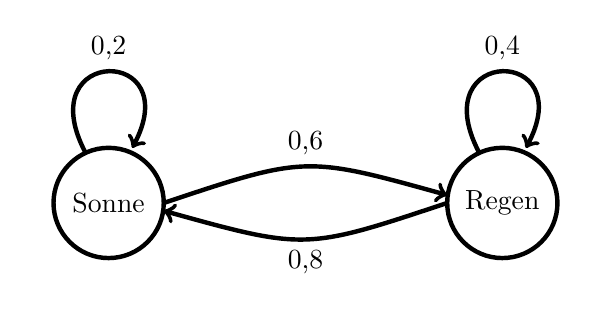
\begin{tikzpicture}	
	\draw[ultra thick] (0,0) circle (0.7cm) node{Sonne};
	\draw[ultra thick] (5,0) circle (0.7cm) node{Regen};
	\draw[->, ultra thick] (0.7,0)..controls(2.5,0.6)..(4.3,0.1) node[midway,above]{0,6};
	\draw[->,ultra thick ](4.3,0)..controls(2.5,-0.6)..(0.7,-0.1)node[midway,below]{0,8};
	\draw[->, ultra thick] (-0.3,0.65)..controls(-1,2) and (1,2)..(0.3,0.7) node[midway,above]{0,2};
	\draw[->, ultra thick] (4.7,0.65)..controls(4,2) and (6,2)..(5.3,0.7) node[midway,above]{0,4};
	\end{tikzpicture}
	\end{center}
	\caption{Übergangsgraph. Knoten geben mögliche Zustände an, Kanten sind Wahrscheinlichkeiten in einen Zustand zu wechseln}
	\label{Markovc}
\end{figure}


	
	\subsection{Hopfield Netze}	
	In diesen Netzen ist jedes Neuron mit allen anderen Neuronen außer sich selber verbunden, wie in Abbildung \ref{HopfieldNetz} dargestellt ist.  Die Neuronen in einem Hopfield Netz sind binär, dass bedeutet, die Ausgabe ist 1, wenn ein Schwellwert $\theta$ überschritten wird, und ansonsten 0.
	\begin{figure}[H]
	\center
	\includesvg[width=5cm]{Hopfield}
	\caption{Modell eines Hopfield Netzes. Alle Neuronen besitzen eine Ein- und Ausgabe und sind über Gewichte jeweils mit allen anderen Neuronen verbunden}
	\label{HopfieldNetz}
	\end{figure}
Die Gewichte in einem Hopfield Netz sind symmetrisch, also gilt $w_{ij} = w_{ji}$. Hopfield Netzen wird eine Energie zugewiesen, die beim Lernen des Netzes minimiert werden soll \cite{Hopfield}:

\begin{equation}
E = -\frac{1}{2}\sum_{i\neq j}{w_{ij}{s_i}{s_j}}+\sum_i{\theta_i\ s_i}
\end{equation}

$s_i$ bzw. $s_j$ sind hierbei die Zustände der Neuronen. Sobald die Energie unverändert bleibt, wurde ein stabiler Zustand erreicht und man befindet sich in einem lokalen Minimum der Energielandschaft.

\subsection{Boltzmann Maschinen}	
Boltzmann Maschinen sind ähnlich wie Hopfield Netze. Ein wesentlicher Unterschied besteht darin, dass die Neuronen stochastisch binär sind, also nicht mehr feuern, wenn ein Schwellwert überschritten ist, sondern mit einer bestimmten Wahrscheinlichkeit eine 1 als Ausgabe haben. Dies wird in der Praxis so realisiert, dass ein Wurf zwischen 0 und 1 größer als die Wahrscheinlichkeit sein muss, um das Neuron zu aktivieren. Boltzmann Maschinen wird auch eine Energie zugewiesen, die ähnlich der von Hopfield Netzen ist \cite{BM}:
\begin{equation}
E = -\left(\sum_{i<j} w_{ij} \, s_i \, s_j + \sum_i \theta_i \, s_i \right)
\end{equation}

Desweiteren werden bei Boltzmann Maschinen die Neuronen in sichtbare und in versteckte Neuronen unterteilt. Die sichtbaren Neuronen haben die Möglichkeit eine Eingabe von außen zu bekommen, die versteckten Neuronen nicht. Der Aufbau ist in Abb. \ref{Boltzmannmaschine} dargestellt.

\begin{figure}[H]
	\center
	\includesvg[width=5cm]{BM}
	\caption{Modell einer Boltzmann Maschine. Gelbe Kreise stellen verstecke Neuronen dar, weiße Kreise sind sichtbare Neuronen.}
	\label{Boltzmannmaschine}
	\end{figure}
	
Die Differenz in der globalen Energie abhängig vom Aktivierungszustand eines Neuron lässt sich als  $\Delta E_i$ beschreiben:

\begin{equation}
\Delta E_i = \sum_j w_{ij} \, s_j + \theta_i
\end{equation}
 Dies lässt sich als Differenz der Energie der beiden möglichen Zustände eines Neurons schreiben:
 \begin{equation}
 \Delta E_i = E_\text{i=off} - E_\text{i=on}
 \end{equation}
 Nun kann man mit Hilfe des Boltzmann Faktors, die Zustände mit ihren relativen Wahrscheinlichkeiten substituieren. Der Boltzmann Faktor ist eine Eigenschaft der Boltzmann Verteilung dass die Energie eines Zustands proportional zur negativen logarithmischen Wahrscheinlichkeit des Zustandes ist:
 
 \begin{equation}
 \Delta E_i = -k_B\,T\ln(p_\text{i=off}) - (-k_B\,T\ln(p_\text{i=on}))
 \end{equation}
 
 Hierbei ist $k_B$ die Boltzmann Konstante und wird in die Temperatur $T$ absorbiert. Unter der Annahme, dass die Wahrscheinlichkeiten für an und aus summiert 1 ergeben müssen kann man die Formel umstellen:
 
 \begin{eqnarray}
 \frac{\Delta E_i}{T} &=& \ln(p_\text{i=on}) - \ln(p_\text{i=off})\\\nonumber
\frac{\Delta E_i}{T} &=& \ln(p_\text{i=on}) - \ln(1 - p_\text{i=on})\\\nonumber
\frac{\Delta E_i}{T} &=& \ln\left(\frac{p_\text{i=on}}{1 - p_\text{i=on}}\right)\\\nonumber
\frac{\Delta E_i}{T} &=& \ln\left(\frac{1 - p_\text{i=on}}{p_\text{i=on}}\right)\\\nonumber
-\frac{\Delta E_i}{T} &=& \ln\left(\frac{1}{p_\text{i=on}} - 1\right)\\\nonumber
\exp\left(-\frac{\Delta E_i}{T}\right) &=& \frac{1}{p_\text{i=on}} - 1
 \end{eqnarray}
Nun kann man die Wahrscheinlichkeit $p_\text{i=on}$ dass Neuron $i$ aktiviert ist ausrechnen:
\begin{equation}
p_\text{i=on} = \frac{1}{1+\exp(-\frac{\Delta E_i}{T})}
\end{equation}

Hierbei ist $T$ die Temperatur des Systems. Diese herleitung bietet die Grundlage für die Verwendung der logistischen Funktion, die zum Beispiel bei eingeschränkten Boltzmann Maschinen verwendet wird \footnote{https://en.wikipedia.org/w/index.php?title=Boltzmann\_ machine\&oldid=665335516}. 

Das Training von Boltzmann Maschinen läuft in zwei Phasen ab: Die erste Phase wird auch als positive Phase bezeichnet und besteht darin, dass man die binären Zustände der sichtbaren Neuronen vorgibt und die Maschine laufen lässt bis sich ein Gleichgewichtszustand (Equilibriumszustand) einstellt, sich also die Aktivierungswahrscheinlichkeiten der einzelnen Neuronen nicht mehr ändern. 

Danach beginnt man mit der negativen Phase. In dieser Phase lässt man die Maschine ohne eine Eingabe von außen laufen bis diese wieder in einem Equilibriumszustand ist. In den Phasen ergeben sich die Verteilungen $P^+(V)$ und $P^-(V)$ über die sichtbaren Neuronen. Das Ziel ist es, die Differenz zwischen beiden Verteilungen zu minimieren. Um die Differenz der beiden Verteilungen zu berechnen, verwendet man die Kullback-Leibler Divergenz \cite{KLD}:
\begin{equation}
G = \sum_{v}{P^{+}(v)\ln\left({\frac{P^{+}(v)}{P^{-}(v)}}\right)}
\end{equation} 
Diese ist immer positiv und und nur dann 0, wenn beide Verteilungen genau gleich sind. Daraus ergibt sich eine einfache Lernregel:
\begin{equation}
\frac{\partial{G}}{\partial{w_{ij}}} = -\frac{1}{R}[p_{ij}^{+}-p_{ij}^{-}]
\end{equation}

Hierbei ist $R$ die Lernrate, und $p_{ij}$ die Wahrscheinlichkeit das Neuron $i$ und $j$ in der positiven, bzw. negativen Phase jeweils aktiviert sind.
Theorethisch wären Boltzmann Maschinen sehr gut in der Lage Modelle von Daten zu trainieren und zu erkennen, allerdings sind diese in der Praxis recht untauglich, da sie bei großen Maschinen zu lange brauchen um trainiert zu werden. Dieses Problem wird mit eingeschränkten Boltzmann Maschinen gelöst.

\subsection{Eingeschränkte Boltzmann Maschinen}	
Bei eingeschränkten Boltzmann Maschinen werden die sichtbaren und versteckten Neuronen als Ebenen betrachtet. Die Ebenen sind symmetrisch miteinander verbunden, jedoch existieren zwischen den Neuronen auf einer Ebene keine Verbindungen wie in Abbildung \ref{RBM} dargestellt.

\begin{figure}[H]
	\center
	\includesvg[width=5cm]{RBM}
	\caption{Modell einer eingeschränkten Boltzmann Maschine. Oben sind die versteckten Knoten und unten die nach außen sichtbaren Knoten.}
	\label{RBM}
	\end{figure}
	
Auch eingeschränkte Boltzmann Maschinen benutzen stochastisch binäre Neuronen wie normale Boltzmann Maschinen.


Als Eingabewerte in so ein Netzwerk sind reelle Werte möglich. Diese würden dann als Aktivierungswahrscheinlichkeiten der sichtbaren Neuronen interpretiert und man müsste dann noch die binären Zustände der sichtbaren Neuronen bestimmen. Im Folgenden wird davon ausgegangen, dass binäre Eingabevektoren vorliegen. 
Eine Konfiguration $(\vec{v},\vec{h})$ aus sichtbaren und unsichtbaren Neuronen wird auch bei eingeschränkten Boltzmann Maschinen eine Energie zugewiesen:

\begin{equation}
E(\vec{v},\vec{h})= - \sum_{i \in visible} a_iv_i- \sum_{j \in hidden} b_j h_j - \sum_{i,j} v_i h_j w_{ij}
\end{equation}

Hierbei sind $v_i$ und $h_j$ die binären Zustände des sichtbaren Knotens $i$ und des versteckten Knotens $j$. $a_i$ und $b_j$ sind die Bias der entsprechenden Knoten und $w_{ij}$ ist das Gewicht zwischen den beiden Knoten. Mit Hilfe dieser Energiefunktion weist das Netz jedem möglichen Paar von sichtbaren und versteckten Knoten eine Wahrscheinlichkeit zu:

\begin{equation}
p(\vec{v},\vec{h})= \frac{1}{Z} e^{-E(\vec{v},\vec{h})}
\end{equation}

Die Zustandssumme (partition function) $Z$ ergibt sich aus der Summe über alle möglichen Werte aus sichtbaren und versteckten Knoten und stellt einen Normierungsfaktor dar, damit die Gesamtwahrscheinlichkeit 1 ergibt:

\begin{equation}
Z=\sum_{\vec{v},\vec{h}} e^{-E(\vec{v},\vec{h})}
\end{equation}

Die Wahrscheinlichkeit, dass sich das Netzwerk einem Eingabebild anpasst, ergibt sich aus der Summe über alle versteckten Vektoren \cite{guide}.

\begin{equation}
p(\vec{v})= \frac{1}{Z} \sum_{\vec{h}} e^{-E(\vec{v},\vec{h})}
\end{equation}

Die Wahrscheinlichkeit, dass sich das Netz einem Trainingsbild anpasst, kann erhöht werden, indem man die Energie der anderen Bilder erhöht. Vor allem für Bilder mit einer niedrigen Energie ist dies wichtig, da diese einen hohen Beitrag zur Zustanddsumme haben. Die Ableitung der Gewichte der logarithmischen Wahrscheinlichkeiten von Trainingsdaten ergibt sich wie folgt:

\begin{equation}
\frac{\partial \log p(\vec{v})}{\partial w_{ij}} = \langle v_ih_j \rangle_{data} - \langle v_i h_j \rangle_{model}
\end{equation}

Hierbei ist $\langle...\rangle$ der Erwartungswert der Verteilung über die Eingabedaten und wird als $data$ bezeichnet. Die vom Netz rekonstruierte Verteilung wird als $model$ bezeichnet. Dies entspricht vom Prinzip her der positiven und der negativen Phase von normalen Boltzmann Maschinen. Auch bei eingeschränkten Boltzmann Maschinen ist das Ziel, dass die Differenz der beiden Verteilungen möglichst gering ist. Sollte diese 0 betragen ist das Modell der Eingabedaten perfekt gelernt, dies geschieht in der Praxis jedoch äußerst selten. Der Erwartungswert ist das Mittel der Wahrscheinlichkeitsverteilung und kann durch das Ziehen von ausreichend vielen Knotenpaaren approximiert werden. Dies führt zu einer einfachen Lernregel für den stochastisch stärksten Aufstieg in der logarithmischen Wahrscheinlichkeit der Trainingsdaten:

\begin{equation}
\Delta w_{ij} = \epsilon\left( \langle v_i h_j \rangle_{data} - \langle v_i h_j \rangle_{model} \right)
\end{equation}

$\epsilon$ ist die Lernrate und kann zur Steuerung, wie stark die Gewichte verändert werden, frei gewählt werden. In der Praxis hat eine zu hohe Lernrate zur Folge, dass die Gewichte zu groß werden und nichts gelernt wird. Eine zu kleine Lernrate führt dazu, dass das Training sehr langsam ist, jedoch empfiehlt es sich für ein besseres Ergebnis gegen Ende des Trainings die Lernrate zu verkleinern \cite{guide}. Da die versteckten Knoten innerhalb einer RBM nicht miteinander verbunden sind, sind diese statistisch voneinander unabhängig. Dies führt dazu, dass man sehr einfach eine Stichprobe ohne Bias für $\langle v_i h_j \rangle_{data}$ erhalten kann. Wenn ein zufällig ausgewähltes Trainingsbild $\vec{v}$ gegeben ist, wird der binäre Zustand $h_j$ jedes versteckten Knotens $j$ mit folgender Wahrscheinlichkeit auf 1 gesetzt:

\begin{equation}
p(h_j = 1 | \vec{v}) = \sigma (b_j + \sum_{i} v_i w_{ij})
\label{ph}
\end{equation}

$\sigma(x)$ ist die logistische sigmoide Funktion $1/(1+e^{-x})$. $v_ih_j$ ist dann eine Stichprobe der Verteilung ohne Bias $a_i$, da die einzelnen versteckten Knoten nicht miteinander verbunden und nur abhängig von den Eingabedaten sind.

Da auch die sichtbaren Knoten keine Verbindungen untereinander haben und damit voneinander unabhängig sind, ist es genau so einfach eine Stichprobe für den Zustand eines sichtbaren Knotens zu erhalten, wenn ein versteckter Vektor $\vec{h}$ gegeben ist:

\begin{equation}
p(v_i =1 | \vec{h}) = \sigma (a_i + \sum_{j} h_j w_{ij})
\label{pv}
\end{equation}

Eine Stichprobe ohne Bias $b_j$ für $<v_i h_j>_{model}$ zu erhalten, ist aufwändiger und kann über abwechselndes "' Gibbs Sampling"' über einen langen Zeitraum berechnet werden. Beim Gibbs Sampling beginnt man mit einem zufälligen Trainingsvektor und hört auf, wenn ein Equilibriumszustand erreicht wird. Eine Iteration des Gibbs sampling besteht daraus, dass man zuerst parallel die Zustände aller versteckten Knoten mit Gleichung \ref{ph} berechnet und im Anschluss mit Gleichung \ref{pv} die sichtbaren Knoten neu berechnet, siehe dazu Abbildung \ref{Markov}

\begin{figure}[H]
	\center
	\includesvg{Markov}
	\caption{Markov-Kette mit Gibbs Sampling. Diese wird mit einem Trainingsvektor initialisiert. Die sichtbaren und unsichtbaren Neuronen werden abwechselnd neu berechnet bis ein Equilibriumszustand erreicht wird.}
	\label{Markov}
	\end{figure}


\subsection{Kontrastive Divergenz}

Ein schnelleres Verfahren als das Gibbs sampling besteht daraus, die Zustände der sichtbaren Knoten mit einem Trainingsvektor zu belegen. Anschließend werden die versteckten Knoten mit Gleichung \ref{ph} berechnet. Nachdem die binären Zustände der versteckten Knoten gefunden sind, wird eine "'Rekonstruktion"' angefertigt indem man jeden sichtbaren Knoten mit einer Wahrscheinlichkeit aus Gleichung \ref{pv} auf 1 setzt. Die Änderung in einem einzelnen Gewicht wird dadurch zu:

\begin{equation}
\Delta w_{ij} = \epsilon \left( \langle v_i h_j\rangle_{data} - \langle v_i h_j \rangle_{recon}\right)
\end{equation}

Diese Lernregel wird Kontrastive Divergenz (Contrastive Divergence(CD)) genannt und liefert bessere Ergebnisse als die vorherige Regel. Zunächst wurde angenommen, dass die  Lernregel grob den Gradienten der logarithmischen Wahrscheinlichkeit approximiert. Danach nahm man an, dass die Differenz zweier Kullback-Leiber Divergenzen approximiert wurden. Was so eine Divergenz ist, wird in \cite{KLD} erklärt und würde hier zu weit führen. Da hierbei ein wichtiger Term jedoch vernachlässigt wird, folgt es auch diesem Gradienten nicht genau und Untersuchungen ergaben, dass die Lernregel gar keinem Gradienten einer Funktion folgt und trotzdem gut funktioniert \cite{noconv}. 

Die Idee hinter Kontrastiven Divergenz besteht darin, dass beim normalen Gibbs Sampling die Markov-Kette sich immer weiter vom gewünschten Modell entfernt, da diese immer unabhängiger von den Eingabedaten wird. Um dem entgegen zu wirken, wird für die Lernregel nicht eine Probe aus dem Gleichgewichtszustand der Boltzmann Maschine verwendet, der entsteht, wenn man das Gibbs Sampling lange genug betreibt, sondern eine Probe aus der rekonstruierten Wahrscheinlichkeitsverteilung nach einem Schritt des Gibbs Sampling. Dies sorgt dafür dass die Markov-Kette näher an der tatsächlichen Wahrscheinlichkeitsverteilung der Eingabe bleibt. Da die rekonstruierte Eingabe näher am Gleichgewichtzustand der Boltzmann Maschine ist als die Eingabe im Gibss Schritt davor, ist garantiert, dass die kontrastive Divergenz niemals negativ wird und nur Null erreicht, wenn das Modell perfekt ist. \cite{digits}

Ein weiterer Schritt, um das Lernen eines Modells auf RBMs zu verbessern, besteht darin, $n$ Schritte des Gibbs samplings zu machen, bevor man die Statistik für $\langle v_i h_j \rangle_{recon}$ ermittelt. Dies wird mit $CD_n$ notiert, wobei $n$ die Anzahl der Schritte des Gibbs samplings angibt.

\section{Deep-Belief Netze}
Deep-Belief Netze sind eine Form von künstlichen neuronalen Netzen. Im Gegensatz zu klassischen Feedforward-Netzen, haben Deep-Belief Netze keine Flache und breite Struktur, sondern, wie der Name schon vermuten lässt, eine tiefe Struktur mit vielen Ebenen.   Diese werden meist unüberwacht trainiert, da angenommen wird, dass Labels zu wenig Informationen enthalten über die vorhandenen Daten oder bei großen Datenmengen sehr oft keine Labels für alle Daten vorhanden sind.  Zum einen ermöglichen Deep-Beielf Netze das Rekonstruieren von einmal trainierten Modellen, z.B. kann ein Deep-Belief Netz, wenn es das Modell von Bildern lernt teile von Bildern oder auch ganze Bilder rekonstruieren. Desweiteren können Deep-Belief Netze zur Klassifikation benutzt werden oder zum Vortrainieren von Feedforward Netzen, da diese nicht so leicht in lokalen Minima stecken bleiben und somit das Netz näher am globalen Minimum konvergiert. Desweiteren macht man sich beim Vortraining zu Nutze, dass man nur wenige Epochen mit Backpropagation lernen muss, da dieser Algorithmus bei tiefen Netzen sehr langsam ist. Zum Trainieren von Deep-Belief Netzen hat sich ein einfacher Algorithmus basierend auf eingeschränkten Boltzmann Maschinen etabliert, der ein effizientes Trainieren der einzelnen Ebenen ermöglicht. 



\subsection{Greedy Algorithmus zum Trainieren von Deep-Belief Netzen}


Ein effizienter Weg ein kompliziertes Modell zu lernen, besteht darin, eine Menge von einfacheren Modellen nacheinander zu lernen. Die Idee des hier vorgestellten greedy Algorithmus besteht darin, dass jedes Modell eine andere Repräsentation der Daten darstellt. Dazu berechnet jedes Modell eine nichtlineare Transformation auf seine Eingabe und die Ausgabe eines Modells wird als Eingabe des nächsten Modells verwendet. 

\begin{figure}[H]
	\center
	\includesvg[width=150pt]{Netzwerk}
	\caption{Hyprid Netzwerk. Die Ebenen $H_3$ und $H_2$ sind mit ungerichteten Kanten verbunden und bilden einen Assoziativspeicher. Die anderen Ebenen sind mit gerichteten Kanten verbunden.}
	\label{Netz}
\end{figure}

In Abbildung \ref{Netz} ist ein generatives Modell mit mehreren Ebenen abgebildet. Als generatives Modell bezeichnet man Modelle, die mit Hilfe von versteckten Parametern zufällige und  beobachtbare Daten generieren, wie zum Beispiel bei einer Markov-Kette. Die oberen beiden Ebenenen kommunizieren über ungerichtete Kanten und simulieren damit unendlich viele weitere gerichtet verbundene Ebenen mit gleichen Gewichten durch die Daten propagiert werden. Das Prinzip wird in Abbildung \ref{Markov} dargestellt, nur dass diesmal jeder neue Schritt als neue Ebene interpretiert wird.  Es gibt keine Verbindungen zwischen den Knoten einer Ebene, sodass diese unabhängig voneinander sind.  Man kann gute Parameter für $W_0$ finden, indem man annimmt, dass die  Gewichte zwischen den höheren Ebenen eine komplementäre Verteilung (complementary prior) abbilden, um den "'Explained Away"'-Effekt für $W_0$ auszulöschen. Dies gilt jedoch nur wenn die Ebenen die gleiche Knotenzahl besitzen, wenn dies nicht der Fall ist, werden die Gewichte der höheren Ebene mit Zufallszahlen einer Gauss-Verteilung initialisiert \cite{learning}.

Der "'Explained Away"'-Effekt beschreibt hierbei dass zwei Knoten stark antikorrelieren, also je höher die Wahrscheinlichkeit in einem Knoten ist, desto geringer ist sie in einem anderen. 
Bildhafter in Abbildung \ref{ExplainedAway} beschrieben ist die Ursache für ein wackelndes Haus durch einen hineinrasenden LKW sehr gering wenn bereits ein Erdbeben das Haus wackeln lässt. Hierbei wäre das wackelnde Haus ein Ausgangsknoten und Erdbeben und der LKW jeweils ein Eingangsknoten. Wenn einer der beiden Eingangsknoten also aktiviert ist, reicht ein Ereignis aus zur Erklärung, da das Eintreten beider Ereignisse sehr unwahrscheinlich ist. Dieses Verhalten macht es schwierig Schlussfolgerungen des Netzes nachzuvollziehen. 

\begin{figure}[H]
	\center
	\includesvg[width=150pt]{ExplainedAway}
	\caption{Beispiel für den Explained Away Effekt. Der Bias von $-10$ am Erdbeben-knoten bedeutet dass dieser ohne beobachtet zu werden $e^{10}$ mal wahrscheinlicher aus als aktiviert ist. Beide Ereignisse zusammen haben eine Wahrscheinlichkeit von $e^{-20}$, da diese unabhängig voneinander sind. Dies ist also sehr unwahrscheinlich. Deshalb erklärt die Aktivierung eines Knotens den anderen weg.}
	\label{ExplainedAway}
\end{figure}

Die Annahme, dass die höheren Ebenen eine komplementäre Verteilung bilden, führt dazu, dass das Lernen von $W_0$ lediglich das Trainieren einer RBM darstellt und mithilfe der Contrastive Divergence eine gute Approximination gefunden wird. Sobald $W_0$ gelernt ist, kann man $W^T_0$, also die transponierte Gewichtsmatrix, als Eingabe für die erste versteckte Ebene benutzen, indem man die Eingabedaten mit dieser multipliziert.

Im allgemeinen findet die eingeschränkte Boltzmann Maschine kein perfektes Modell für die Eingabedaten. Das Modell kann durch einen einfachen greedy Algorithmus verbessert werden:
 
\begin{enumerate}
\item Lerne $W_0$.
\item Benutze $W_0^T$ um die Verteilung der einzelnen Variablen in der ersten versteckten Ebene zu approximieren.
\item Lerne eine weitere eingeschränkte Boltzmann Maschine  mithilfe der "'Daten"', die durch $W_0^T$ generiert wurden, für die nächste Ebene.
\end{enumerate}



Jede durch den Algorithmus trainierte Ebene verbessert das Modell. Gleichzeitig bedeutet dies auch, dass jedes Modell durch Hinzufügen von neuen Ebenen bis zu einem bestimmten Punkt verbessert werden kann, wenn man jede Ebene sorgfältig genug trainiert. Wenn alle Ebenen die gleiche Anzahl von Knoten haben, besteht eine Verbesserung darin, dass jede neue Ebene mit den bereits gelernten Gewichten initialisiert wird \cite{learning}. Bei unterschiedlicher Knotenzahl werden die Gewichte mit Zufallszahlen initialisiert.

\subsection{Deep-Belief Netze zur Klassifikation}
Nachdem man das Netz mit dem im vorigen Kapitel beschriebenen Algorithmus trainiert hat, muss man immer noch die Labeldaten ins Netz speisen wenn man dieses für eine Klassifikation nutzen möchte. Dazu gibt es im wesentlichen zwei verschiedene Methoden:

Die erste Methode besteht darin, beim Training auf der vorletzten Ebene eine Gruppe von Softmax-Neuronen hinzuzufügen. Diese haben eine andere Aktivierungsfunktion als die normalen Neuronen: 
\begin{equation}
p_j = \frac{e^{x_j}}{\sum_{i=1}^K e^{x_i}}
\end{equation}

Diese Aktivierungsfunktion sorgt dafür, dass die Aktivierung eines Neurons von der Aktivierung der anderen Neuronen abhängig ist und somit immer nur ein Neuron in der Gruppe aktiviert ist. Indem man abhängig vom Label ein Neuron fest auf 1 setzt beim Trainieren, lernt das Netz welche Aktivierungszustände zu einer Klasse gehören. Dieses Training ist unüberwacht. Der Netzaufbau für diese Art der Klassifikation wird in Abbildung \ref{SMTrain} gezeigt. Wenn man nach dem Training einen Datensatz durchs Netz propagiert und anschließend ein paar Gibbs Samplings zwischen den letzten beiden Ebenen macht, kann man in der Softmax Gruppe das erkannte Label ablesen.
\begin{figure}[H]
	\center
	\includesvg[width=200pt]{SMTrain}
	\caption{Netzwerk mit Softmax-Gruppe zum Klassifizieren. Aus Sicht von $H_3$ werden die Softmax-Neuronen als normale Eingabe betrachtet. An der Softmax-Gruppe kann später die gefundene Klasse abgelesen werden.}
	\label{SMTrain}
\end{figure}

Die zweite Methode besteht darin, dass Deep-Belief Netz normal zu trainieren und nach dem Training eine Ebene mit Ausgabenneuronen an die letzte Ebene hinzuzufügen. Diese Neuronen können entweder die sigmoide Funktion als Aktivierung nutzen oder auch eine Softmax Gruppe bilden. Nun trainiert man die Gewichte zwischen der neuen Ebene und der letzten Ebene mit Backpropagation um die Labelinformationen mit den Aktivierungszuständen des Netzes zu verbinden. Der Aufbau des so enstandenen Netzes wird in Abbildung \ref{BPTrain} gezeigt. Um das Ergebnis im Anschluß noch weiter zu verbessern, kann man die Gewichte des ganzen Netzes nochmals mit Backpropagation feiner einstellen, allerdings sollte das Netz auch ohne diesen Schritt bereits positive Ergebnisse liefern\cite{backprop}.

\begin{figure}[H]
	\center
	\includesvg[width=4cm]{BPTrain}
	\caption{Netzwerk mit Ausgabeschicht zur Klassifizierung. Die Gewichte zwischen $H_3$ und der Ausgabe werden mit Backpropagation trainiert.}
	\label{BPTrain}
\end{figure}


\section{Implementation}
Dieses Kapitel behandelt das verwendete Framework, welches in der Bachelorabeit von Evgenij Helm entstanden ist \cite{Helm}. Zunächst wird der allgeime Aufbau und die Verwendung beschrieben und später welche Erweiterungen für diese Arbeit hinzugefügt wurden.
\subsection{Allgemeiner Aufbau des Frameworks}
\begin{figure}[H]
	\center
	\includesvg{Aufbau}
	\caption{Klassenherarchie des verwendeten Frameworks, rot umrandete Klassen wurden in dieser Arbeit hinzugefügt.}
	\label{Aufbau}
\end{figure}

Die verschiedenen Klassen des Frameworks sind in Abbildung \ref{Aufbau} dargestellt. In der Grundversion kann das Framework Feedworward-Netze einmal mit der Backpropagation trainieren und mit einem genetischen Algorithmus welcher in \cite{Helm} erklärt wird. Beim aufrufen des Programms stehen verschiedene Parameter zur Steuerung des Verhaltens zur Verfügung:
\begin{itemize}
\renewcommand\labelitemi{--}
\item N [Pfad]: Liest die Konfiguration für das zu Verwendende neuronale Netz ein. Eine mögliche Konfiguration kann so aussehen:
\begin{lstlisting}[caption={Beispielkonfigurationsdatei für ein neuronales Netz},captionpos=b, label=NNKonf]
#Linear=0,SIGMOID=1,TANH=2,LECUN_TANH=3, BINARY=4, SOFTMAX=5
FunctionType=1
LastLayerFunction=5
#NONE=0, UNIFORM=1, LECUN=2, NORMAL0=3
WeightInitType=1
LayerCount=3
SoftmaxGroup=1
#Anzahl der Neuronen pro Layer : {Input},{Hidden_0},...,{Output}
LayerNeuronCount=4,4,2

\end{lstlisting} 
Zeilen die mit einem \# beginnen werden nicht ausgelesen und gelten als Kommentar. FunctionType gibt an, welche Aktivierungsfunktion für die einzelnen Neuronen verwendet werden sollen. Dieser Parameter wird bei Deep-Belief Netzen ignoriert, da diese grundsätzlich stochastisch binär aktiviert werden. In der Beispieldatei in Listing \ref{NNKonf} wäre dies die logistische Funktion. LastLayerFunction gibt an welche Aktivierungsfunktion auf der Ausgabeebene verwendet werden soll. Im Beispiel würde hier die Softmaxfunktion verwendet werden. WeightInitType spezifiziert mit welcher Verteilung die Gewichte des neuronalen Netzes initialisiert werden und wäre hier eine Gleichverteilung zwischen $-1$ und $1$. LayerCount gibt die Anzahl der Ebenen des Netzes an, inklusive Eingabe- und Ausgabeebene. SoftmaxGroup ist nur für Deep-Belief Netze relevant und gibt die größe der Softmaxgruppe an, wenn diese auf die vorletzte Ebene gesetzt wird. LayerNeuronCount gibt die Anzahl der Neuronen pro Ebene an. Im Beispiel hätte das Netz vier Eingabeneuronen, vier versteckte Neuronen und zwei Ausgabeneuronen.
\item D [Pfad]: Gibt den Pfad zu den Trainingsdaten an. Wenn es keine zusätzlichen Testdaten gibt, muss mit -K angegeben werden, in wieviele Teile der Datensatz aufgeteilt werden soll. Listing \ref{DatenConf} zeigt Auszüge aus einem Datensatz
\begin{lstlisting}[caption= {Auszug aus einem der verwendeten Datensätze}, captionpos=b, label={DatenConf}]
1346 4 1
0.1395 0.1008 0.2407 0.9230
0
0.5489 1.0000 0.4926 0.4605
1
0.1892 0.0184 0.3687 0.8308
1
...
...
\end{lstlisting}
Ein Datensatz enthält in der ersten Zeile die Anzahl der Daten, wie viele Eingabewerte es gibt und wie viele Ausgabewerte es gibt. Dies wäre in Listing \ref{DatenConf} 1346 einzelne Datensätze mit 4 Parametern als Eingabe und einem Wert als Ausgabe. 
\item TD [Pfad]: Gibt den Pfad zu zusätzlichen Testdaten an. Das Format für Testdaten entspricht dem Format für Trainingsdaten. Hierbei ist vom Benutzer darauf zu achten, dass die angegebenen Testdaten zu den Trainingsdaten gehören, da dies nicht vom Programm überprüft wird.
\item B [Pfad]: Gibt den Pfad zur Konfigurationsdatei für die Backpropagation an. 
\begin{lstlisting}[captionpos=b,caption={Beispielkonfiguration für den Backpropagation-Algorithmus},label={BPConf}]
ErrorThreshold=0
MaxLoopCount=1000
BatchSize=1
Alpha=0.5
Momentum=0.0
DecayRate=0
\end{lstlisting}
Die Konfigurationsdatei enthält verschiedene Parameter für die Backpropagation und wird in Listing \ref{BPConf} gezeigt. ErrorThreshold gibt an, ab welchem MSE der Algorithmus aufhört falls noch nicht alle Epochen trainiert wurden. MaxLoopCount gibt an, wieviele Epochen trainiert werden sollen. Batchsize definiert die Anzahl von Trainingssätzen pro Batch. Alpha bestimmt die Lernrate und Momentum das Momentum. Das Lernen mit Momentum wird in \cite{Helm} erklärt. DecayRate gibt an, wie die Lernrate während des Trainings angepasst wird. Bei 0 bleibt die Lernrate unverändert.

\item CD[Pfad]: Gibt Pfad zur Konfigurationsdatei der Kontrastiven Divergenz an. 
\begin{lstlisting}[captionpos=b,caption={Beispielkonfiguration der Kontrastiven Divergenz},label={CDConf}]
GibbsSteps=1
BatchSize=50
LearnRate=0.5
Epochs= 100
\end{lstlisting}
In Listing \ref{CDConf} wird eine mögliche Konfiguration der Kontrastiven Divergenz gezeigt. GibssSteps gibt an, wie viele Schritte des Gibbs Samplings verwendet werden sollen. BatchSize gibt die Anzahl der Daten pro Batch an. LearnRate steuert die Lernrate des Algorithmus und Epochs gibt die Anzahl der Epochen an.

\item G [Pfad]: Gibt den Pfad zur Konfigurationsdatei für den genetischen Algorithmus an. Dieser wird in \cite{Helm} erklärt und ist nur für die Vollständigkeit hier aufgeführt.
\item SW [Pfad]:	Speicherung der Gewichte nach dem Training. Die
			Variablen \%N, \%B, \%G,  \%D in [Pfad] werden mit dem 
 			jeweiligen Dateinamen des Parameters ersetzt.
			\%K wird mit dem Iterationsschritt 0...K-1 ersetzt.
\item SR [File]:	Speichern der Ergebnisse für MSE und die Dauer des jeweiligen Trainings mit Angabe des Iterationsschrittes. Varibalen werden wie bei -SW ersetzt. 

\item C [Wert]: Gibt einen Wert an, um den bei den Testdaten vom gewünschten Ergebnis abgewichen werden darf. Größere Abweichungen werden als falsch bewertet. Muss immer mit angegeben werden, wird jedoch bei mehr als einem Ausgabeneuron beim Testen ignoriert.

\item K [Wert]: Aktiviert die Kreuzvalidierung. Der Wert gibt an, in wieviele Teile der Datensatz aufgeteilt werden soll. Das Netzwerk wird mit Wert-1 teilen trainiert und dem übrig gebliebenen Teil getestet. Falls die Daten nicht glatt durch den Wert teilbar sind, werden die restlichen Daten zum Testen verwendet. 

\item O [Wert]:	Offset der beim Speichern auf die Zeit addiert wird.
\item I [Wert]: Anzahl der Wiederholungen des Trainings. Anschließend werden Mittelwert und Streuung über alle Testergebnisse berechnet.
\end{itemize}

\subsection{Erweiterungen des Frameworks}
Das Framework wurde erweitert, sodass dieses nun auch Deep-Belief Netze trainieren kann. Die dafür hinzugefügten Klassen sind in Abbildung \ref{Aufbau} rot markiert.

Die Klasse ContrastiveDivergenceConfig liest die Parameter für die Kontrastive Divergenz aus einer Datei ein. Die Klasse kann einfach erweitert werden und setzt momentan die Anzahl der Gibbsschritte, die Anzahl der Epochen, die Lernrate und die Größe der zu trainierenden Batches.

DBNLayer erweitert die Layerklasse soweit, dass statt normalen Neuronen Neuronen für das Deep-Belief-Netz benutzt werden und neben den rückwärtsgerichteten Gewichten der normalen Neuronen auch vorwärtsgerichtete Gewichte besitzt. Diese Gewichte stellen jedoch lediglich Zeiger auf die rückwärtsgerichteten Gewichte dar. Desweiteren wurde eine Möglichkeit geschaffen die Gewichte für das Deep-Belief Netz zu initialiseren. Dazu wird für jedes Gewicht eine zufällige Zahl einer gausschen Normalverteilung mit einem Erwartungswert von 0 und einer Standardabweichung von $0,1$ gezogen.

DeepBeliefNet stellt die Netzstruktur für Deep-Belief Netze zur Verfügung. Im Gegensatz zu den normalen Netzwerken des Frameworks, besitzen Deep-Belief Netze auch auf der Eingabeebene eigene Neuronen. Dies ist wichtig, da man für die Kontrastive Divergenz die Aktivierungswahrscheinlichkeiten der einzelnen Neuronen speichern muss. Desweiteren besitzt das Netz die Funktion seine Gewichte so abzuspeichern, dass diese von einem normalen neuronalen Netz wieder eingelesen werden können. Dabei gehen die Biasgewichte in Rückwärtsrichtung verloren, da diese von dem normalen neuronalen Netz mit Backpropagation nicht benötigt werden.

DBNNeuron ist eine Erweiterung der Neuron Klasse. DBNNeuronen können ihre Aktivierungswahrscheinlichkeit speichern und besitzen die Möglichkeit auf die Gewichte zum nächsthöheren Layer zuzugreifen. Außerdem kam eine Funktion zum Initialisieren von Biasgewichten hinzu. Diese bekommt entweder den Datencontainer für die Eingabedaten des Layers oder NULL übergeben. Wenn kein Container übergeben wird, wird der Bias auf 0 gesetzt. Dies ist der Fall, wenn der Biasknoten für die versteckte Ebene zuständig ist. Wenn ein Container übergeben wird, wird aus den Eingabedaten der Initialwert des Bias für jeden sichtbaren Knoten $i$ berechnet:
\begin{equation}
\log [p_i/(1-p_i)]
\end{equation}
$p_i$ ist hierbei die durchschnittliche Aktivierungswahrscheinlichkeit des Knoten $i$ über alle Eingabedaten.

Als letzte wichtige Erweiterung wurde die Klasse ContrastiveDivergence implementiert, diese enthält den Lernalgorithmus für das Deep-Belief Netz.
\begin{figure}[H]
\begin{algorithm}[H]
 \KwData{Eingabedaten, Epochenanzahl, Anzahl der Gibsschritte, Lernrate}
 \KwResult{Traniertes Deep Belief Netz}
 Initialisiere leere Datencontainer für Eingabedaten für jede Ebene\\
 \For{jede Ebene}{
 	Initialisiere Bias für versteckte Ebene mit 0\\
 	Initialisiere Bias für sichtbare Ebene mit $\log [p_i/(1-p_i)]$\\
 	\For{Jeden Datensatz}{
	Setze Eingabedaten als Aktivierungswahrscheinlichkeit für sichtbare Ebene\\
	Bestimme Aktivierungen der sichtbaren Knoten\\
	Berechne Wahrscheinlichkeiten für versteckte Knoten: $ p(h_j = 1 | \vec{v}) = \sigma (b_j + \sum_{i} v_i w_{ij})$\\
	Sammle Statistik für $\langle v_i h_j\rangle_{data}$
	
	\For {Anzahl Gibbsschritte}{
	Berechne Wahrscheinlichkeiten für sichtbare Knoten: $	p(v_i =1 | \vec{h}) = \sigma (a_i + \sum_{j} h_j w_{ij})$\\
	Berechne Wahrscheinlichkeiten für versteckte Knoten
	}
	Sammle Statistik für $\langle v_i h_j\rangle_{model}$\\
	Passe Gewichte an: $w_{ij}=w_{ij} +\epsilon \left( \langle v_i h_j\rangle_{data} - \langle v_i h_j \rangle_{recon}\right)$\\
	Passe Bias für sichtbare Knoten an: $a_i = a_i +\epsilon \left( \langle v_i\rangle_{data} - \langle v_i\rangle_{recon}\right)$\\
	Passe Bias für versteckte Knoten an: $b_i = b_i +\epsilon \left( \langle h_i\rangle_{data} - \langle h_i\rangle_{recon}\right)$\\
 	}
 	\For{Jeden Datensatz}{
 	Propagiere Eingabedaten durch trainierte Ebene und speichere Ergebnis in Datencontainer für die nächste Ebene\\
 	}
 }
 \caption{Implementation der Kontrastiven Divergenz}
\end{algorithm}
\end{figure}


Im Anschluss an die Kontrastive Divergenz werden die Gewichte zwischen der Ausgabe- und der vorletzten Ebene mit Hilfe von Backpropagation traniert.

Das Framework reagiert auf verschiedene Eingabeparameter zum Setzen von Konfigurationsdaten für den Aufbau des Netzes und welcher Lernalgorithmus verwendet werden soll. Wenn neben einer Konfiguration für die Kontrastive Divergenz auch eine Konfiguration für die Backpropagation angegeben ist, wird das Netz im Anschluss nochmal feiner trainiert.

\section{Versuch}
Es sollen die verschiedenen Methoden zum Klassifizieren von Dateneingaben mit Deep-Belief Netzen untersucht werden. Dazu werden verschiedene Netzgrößen mit ansonsten den gleichen Parametern getestet. Zur Verfügung stehen zwei verschiedene Datensätze.
\subsection{Achsensymmetrie und Rotationssymmetrie}
Die erste Datenbank besteht aus 1346 Datensätzen und beinhaltet Merkmale zu einzelnen Punkten. Der Datensatz wurde von  Prof. Dr. Christoph Dalitz zur Verfügung gestellt. Jeder Datensatz enthält vier Merkmale zu einem einzelnen Punkt. Dieser Punkt ist entweder der Kategorie Achsensymmetrisch oder Rotationssymetrisch zugeordnet. Die einzelnen Klassen wurden mit 1 und 0 kodiert. Die vier Merkmale sind auf das Intervall $[0,1]$ skaliert. Für jedes Merkmal gibt es ein Eingabeneuron und jede Klasse hat ein Ausgabeneuron. Aufgrund fehlender Testdaten wird eine einfache Kreuzvalidierung mit $K=5$ gewählt.  Daraus ergibt sich für jeden Trainingsdatensatz eine Größe von 1076 und jeder Testdatensatz besteht aus 270 Datensätzen.

\subsection{MNIST Datenbank}
Die Mixed National Institute of Standards and Technology\footnote{http://yann.lecun.com/exdb/mnist/} beinhaltet 70000 Datensätze. Diese Datenbank ist ein Standarddatensatz zum Vergleichen von verschiedenen Verfahren der Mustererkennung und bietet daher eine große Vergleichsmöglichkeit. Der Datensatz besteht aus 60000 Trainingsdaten und 10000 Testdaten. Die Daten bestehen aus $28 \cdot 28$ Grauwertpixeln und ergeben damit eine Eingabe von 784 Neuronen. Da die Bilder zur Erkennung von Ziffern sind ergeben sich 10 Ausgabeneuronen, für jede Klasse ein Neuron. Das Ziel ist es, dass das Neuron zu dem die Klasse des Bildes gehört aktiviert wird und die anderen Neuronen nicht. Zur Eingabe ins Netz wurden die Grauwerte auf das Intervall $[0,1]$ skaliert.

\subsection{Versuchsdurchführung}
Die beiden Datenbanken werden mit verschiedenen Topologien getestet. Als Grundlage werden die Ergebnisse des Backpropagation Algorithmus verwendet und diese dann mit dem Vortraining durch Kontrastive Divergenz verglichen und mit einem Deep-Belief Netz mit einer Softmax Gruppe. Da es zu Aufwändig ist, alle möglichen Netztopologien zu testen, werden nur ein paar Stichpropen ausprobiert.

\subsubsection{Achsensymetrie und Rotationssymetrie}
Bei diesem Datensatz werden Topologien mit 1-2 versteckten Ebenen und verschiedenen Anzahlen von Neuronen auf den versteckten Ebenen untersucht. Für die Backpropagation wird eine Epochenanzahl von 1000 gewählt mit einer Lernrate von 0,5. Die Kontrastive Divergenz hat eine Epochenanzahl von 100 und eine Lernrate von 0,1. Es wird ein Gibbs Schritt verwendet. Für das Trainieren der letzten Ebene nach der Kontrastiven Divergenz wird eine Epochenanzahl von 1000 und eine Lernrate von 0,1 verwendet. In Tabelle \ref{sigmoid} sieht man....
\begin{table}[H]


\begin{tabularx}{\textwidth}{|c|c|X|X|X|X|X|X|}
	\hline
	NR & Topologie & \multicolumn{3}{|c|}{Backpropagation} & \multicolumn{3}{|c|}{BP mit Vortraining} \\\hline
	&&MSE& Fehler&Laufzeit&MSE& Fehler&Laufzeit
	\\\hline
	1&4-2-1&&&&&&\\\hline
	2&4-4-1&&&&&&\\\hline
	3&4-6-1&&&&&&\\\hline
	4&4-8-1&&&&&&\\\hline
	5&4-2-2-1&&&&&&\\\hline
	6&4-4-4-1&&&&&&\\\hline
	7&4-4-8-1&&&&&&\\\hline
	8&4-8-8-1&&&&&&\\\hline
	\end{tabularx}
	\caption{Vergleich verschiedener Netztopologien mit einem Ausgabeneuron}
	\label{sigmoid}
	\end{table}
	
	
	
	In den Arbeiten zu Deep-Belief Netzwerken wurden für die Backpropagation Softmaxneuronen als Ausgabeneuronen um ein besseres Ergebnis zu liefern. Daher wurde ein weiterer Versuch durchgeführt. Dieser Vergleicht auch ein Deep-Belief Netz mit einer Softmax Gruppe in der vorletzten Ebene die auch als Ausgabe verwendet wird.

\begin{table}[H]
\begin{tabularx}{\textwidth}{|c|c|X|X|X|X|X|X|}
	\hline
	NR & Topologie & \multicolumn{2}{|c|}{Backpropagation} & \multicolumn{2}{|c|}{BP mit Vortraining} & \multicolumn{2}{|c|}{DBN mit Softmax Gruppe}\\\hline
	&&MSE& Fehler&MSE& Fehler&MSE& Fehler
	\\\hline
	1&4-2-2&&&&&&\\\hline
	2&4-4-2&&&&&&\\\hline
	3&4-6-2&&&&&&\\\hline
	4&4-8-2&&&&&&\\\hline
	5&4-2-2-2&&&&&&\\\hline
	6&4-4-4-2&&&&&&\\\hline
	7&4-4-8-2&&&&&&\\\hline
	8&4-8-8-2&&&&&&\\\hline
	\end{tabularx}
	\caption{Vergleich verschiedener Netztopologien mit Softmax-Neuronen als Ausgabe}
	\end{table}
	\subsubsection{MNIST Datenbank}
	
	Bei der MNIST Datenbank wird zunächst die in \cite{learning} verwendete Toplogie gestestet und mit dem Ergebnis der Arbeit verglichen. Da diese nur den relativen Fehler enthält, wird hier auch nur dieser gemessen. Diese Topologie besteht aus 5 Ebenen. Die erste Ebene hat 784 Eingabeknoten für die Bilddaten. Danach kommen drei versteckte Ebenen mit 500,500 und 2000 Knoten und eine Ausgabeebene mit 10 Knoten zur Klassifizierung. Dabei wurde die Anzahl der Gibbs Schritte variiert und auf 1, 10 und 30 gesetzt. Eine Frage die sich stellt ist, ob die dritte versteckte Ebene mit 2000 Knoten so groß sein muss, oder ob das Netz auch mit weniger Knoten auskommt. Daher wurden noch zwei Topologien mit 1000 bzw. 500 versteckten Knoten getestet.
	\begin{table}[H]
\begin{tabularx}{\textwidth}{|c|c|c|c|X|}
	\hline
	NR & Topologie &Gibbs Schritte& BP mit Vortraining & DBN mit Softmax Gruppe
	\\\hline
	1&784-500-500-2000-10&1&&\\\hline
	2&784-500-500-2000-10&10&&\\\hline
	3&784-500-500-2000-10&30&&\\\hline
	4&784-500-500-1000-10&1&&\\\hline
	5&784-500-500-500-10&1&&\\\hline
	\end{tabularx}
	\caption{Vergleich verschiedener Netztopologien mit Softmax-Neuronen als Ausgabe}
	\end{table}
	
	\section{Probleme von Deep-Belief Netzen}
	Deep-Belief Netze trainieren tiefe Netze zwar schneller als die Backpropagation, allerdings dauert das Training bei großen Ebenen immer noch sehr lange. Eine wichtige Frage ist hierbei, ob die einzelnen Ebenen so groß sein müssen oder ob kleinere Ebenen zu einem gleichen oder sogar besseren Ergebnis führen können. Eine weiteres Problem ist durch den Explained-away Effekt, dass man von außen sehr schlecht nachvollziehen kann, wie das Netz zu einer bestimmten Entscheidung kommt. Generell scheint es durch die Menge der einstellbaren und möglichen Parameter für ein solches Netz unmöglich zu sein eine optimale Einstellung der einzelnen Parameter zu finden ohne diese langwierig einzelnd ausprobieren zu müssen. 

\subsection{Einfache Verbesserung}
Eine einfache Verbesserung um die Anzahl der Neuronen auf den einzelnen Ebenen zu reduzieren, besteht darin, Neuronen die bei jedem Trainingsmuster immer aktiviert bzw. nicht aktiviert sind aus dem Netz zu entfernen. Dies sollte theorethisch kein Problem darstellen, da der Bias dieser Knoten diese ohnehin schon für die weiteren Berechnungen unwichtig macht. Diesen Schritt könnte man nach dem Training einer Ebene ausführen und so die Neuronenzahl etwas reduzieren.


\newpage
\begin{thebibliography}{9}
\bibliographystyle{unsrt}
\bibitem{BM}
G. E. Hinton, T. J. Sejnowski,
\emph{Learning and relearning in Boltzmann machines}, 
Parallel Distributed Processing: Explorations in the Microstructure of Cognition. Volume 1: Foundations, MIT Press, Seite 282-317, 1986

\bibitem{guide}
Geoffrey Hinton,
\emph{A Practical Guide to Training Restricted Boltzmann Machines},
Department of Computer Science, 
University of Toronto,
2010

\bibitem{digits}
Geoffrey Hinton,
\emph{Training Products of Experts by Minimizing Contrastive Divergence},
Neural Computation 14 Seite 1771-1800,
2002

\bibitem{noconv}
Ilya Sutske, Tijmen Tieleman,
\emph{On the convergence properties of contrastive divergence},
Proceedings of the 13th International Conference on Artificial Intelligence and Statistics (AISTATS),
2010 
\bibitem{learning}
Geoffrey Hinton, Yee-Whye Teh,
\emph{A Fast Learning Algorithm for Deep Belief Nets},
Neural Computation 18 Seiten 1527-1554,
2006

\bibitem{backprop}
G. E. Hinton, R. R. Salakhutdinov,
\emph{Reducing the dimensionality of data with neural networks},
Science Vol. 313. no. 5786n Seite 504 - 507,
2006

\bibitem{Hopfield}
J. J. Hopfield,
 \emph{Neural networks and physical systems with emergent collective computational properties},
Proceedings of the National Academy of Sciences (USA) 79, Seite 2554-2558,
1982

\bibitem{KLD}
 S. Kullback, R.A Leibler,
\emph{On information and sufficiency},
Annals of Mathematical Statistics 22 No. 1,
Seite  79–86,
 1951
 
\bibitem{PDP} David E. Rumelhart, James L. McClelland: {\em Parallel Distributed Processing Explorations in the microstrucutre of Cognition Volume 1: Foundations}, A Bradford Book, 1987

\bibitem{bachelor} 
M. Kämmerer, \emph{Implementation eines Neuronalen Netzes auf Graphikkarten für Anwendungen in der Hochenergiephysik}, Hochschule Niederrhein, 2013

\bibitem{Helm} 
E. Helm, \emph{Back-Propagation Algorithmus und genetische
Algorithmen zum Training neuronaler Netze
}, Hochschule Niederrhein, 2014

\bibitem{Markovchains}
A. Blake, P. Kohli, C. Rother,
\emph{Markov Random Fields for Vision and Image Processing}
, MIT Press, 2011

\end{thebibliography}
\newpage
\listoffigures


\end{document}

















































